\begin{figure}[h!]
\centering
%
\begin{subfigure}{0.25\textwidth}
  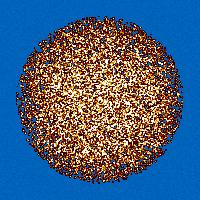
\includegraphics[width=0.95\linewidth]{figures/burn-20-bstep0}
  \caption{Fresh}
  \label{fig:bstep0}
\end{subfigure}%
%
\begin{subfigure}{0.25\textwidth}
  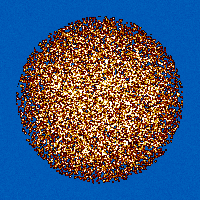
\includegraphics[width=0.95\linewidth]{figures/burn-20-bstep1}
  \caption{One Pass}
  \label{fig:bstep1}
\end{subfigure}%
%
\begin{subfigure}{0.25\textwidth}
  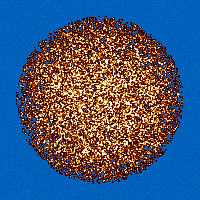
\includegraphics[width=0.95\linewidth]{figures/burn-20-bstep2}
  \caption{Two Passes}
  \label{fig:bstep2}
\end{subfigure}%

\begin{subfigure}{0.25\textwidth}
  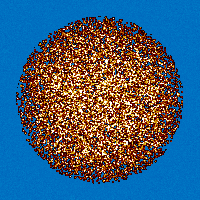
\includegraphics[width=0.95\linewidth]{figures/burn-20-bstep3}
  \caption{Three Passes}
  \label{fig:bstep3}
\end{subfigure}%
%
\begin{subfigure}{0.25\textwidth}
  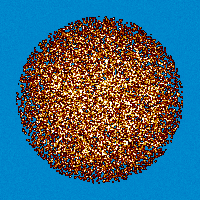
\includegraphics[width=0.95\linewidth]{figures/burn-20-bstep4}
  \caption{Four Passes}
  \label{fig:bstep4}
\end{subfigure}%
%
\begin{subfigure}{0.25\textwidth}
  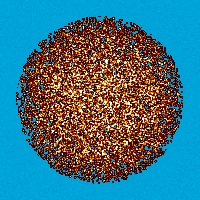
\includegraphics[width=0.95\linewidth]{figures/burn-20-bstep5}
  \caption{Five Passes}
  \label{fig:bstep5}
\end{subfigure}%

\begin{subfigure}{0.25\textwidth}
  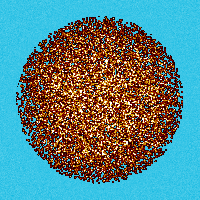
\includegraphics[width=0.95\linewidth]{figures/burn-20-bstep6}
  \caption{Six Passes}
  \label{fig:bstep6}
\end{subfigure}%
%
\caption{Mesh Figures For Single Pebble Burnup}
\label{fig:burn-meshes}
\end{figure}